\documentclass[12pt]{report}

\usepackage[language=english, type=bachelor]{style}
\usepackage{amsmath}
\usepackage{amssymb}
\usepackage{listings}
\usepackage{pmboxdraw}
\usepackage{newunicodechar}
\newunicodechar{ş}{\c{s}}
\newunicodechar{ș}{\c{s}}
\newunicodechar{ţ}{\c{t}}
\newunicodechar{ț}{\c{t}}
\newunicodechar{ă}{{\u{a}}}
\newunicodechar{â}{{\^{a}}}
\newunicodechar{î}{{\^{\i}}}
\newunicodechar{■}{$\blacksquare$}
\newunicodechar{←}{$\leftarrow$}
\newunicodechar{≠}{$\neq$}
\newunicodechar{≤}{$\leq$}
\newunicodechar{≥}{$\geq$}
\newunicodechar{√}{$\surd$}
\usepackage{tikz}
\usetikzlibrary{shapes.geometric, arrows.meta, positioning, fit, backgrounds}

\usepackage{fancyhdr}
\pagestyle{fancy}
\lhead{}
\chead{}
\renewcommand{\headrulewidth}{0.2pt}
\renewcommand{\footrulewidth}{0.2pt}

\begin{document}

\specialization{Computer Science}
\title{Pseudo++: A Comprehensive Pseudocode Toolchain for Romanian High School Computer Science}
\author{Bujor Mihai Alexandru}
\supervisor{Assoc. Prof. Rareș Florin Boian, PhD}

\maketitle

\newpage
\thispagestyle{empty}
\mbox{}
\newpage
\pagenumbering{roman}

\cleardoublepage
\chapter*{Abstract}
\addcontentsline{toc}{chapter}{Abstract}
\vspace{0.5cm}
\hrule
\vspace{0.5cm}

The Romanian national baccalaureate examination in Computer Science requires
candidates to read, write, and reason about programs expressed in a pseudocode
dialect that uses Romanian keywords, Unicode mathematical symbols, and a
box-drawing block structure.  Despite being central to the curriculum, this
dialect has no standard execution environment: students must trace programs
by hand, with no automated way to verify correctness.

This thesis presents \textbf{Pseudo++}, an open-source toolchain that fills
this gap.  The toolchain is built around a single C library compiled to both
a native binary and a WebAssembly module, ensuring identical behaviour across
all interfaces.  On the language side, a grammar, formatter, and linter
define, normalise, and statically analyse the dialect.  For execution, an
interpreter and debugger let students run and inspect programs.  A transpiler
targeting C, C++, and Pascal bridges pseudocode to real languages, while a
loop-equivalence module makes the semantic equivalence between the different
loop forms easier to grasp.  All of this is delivered through a browser-based
editor that works entirely offline and a command-line interface.

The web editor requires no installation and has no server-side component,
making it accessible in school lab environments.  Self-hosting requires only
serving the static release bundle as a directory of files.  Pseudo++ is
the only tool that combines execution, debugging, transpilation, and linting
for the Romanian baccalaureate pseudocode dialect in a single browser-based
environment.


\tableofcontents

\newpage
\pagenumbering{arabic}

\chapter{Introduction}
\label{chap:introduction}

\section{Problem Statement}
\label{sec:problem}

\section{Motivation}
\label{sec:motivation}

\section{Related Work}
\label{sec:related-brief}

\section{Contributions}
\label{sec:contributions}

\section{Thesis Structure}
\label{sec:structure}

\chapter{Related Work}
\label{chap:related}

This chapter surveys tools and research that overlap with one or more
aspects of the Pseudo++ toolchain: general-purpose online execution
platforms, pseudocode-specific interpreters, visual programming
environments, and the use of transpilation in educational settings.
Each category is assessed along the dimensions relevant to the Romanian
baccalaureate use case, and Section~\ref{sec:comparison} closes with a
direct feature comparison.

% ─────────────────────────────────────────────────────────────────────────────
\section{Online Code Execution Platforms}
\label{sec:online-editors}

The most commonly used tools in Romanian high-school computer science
classes are browser-based programming environments for the two target exam languages,
C++ and Pascal.  Platforms such as Replit \cite{replit} and OnlineGDB
\cite{onlinegdb} provide a full edit-compile-run loop in the browser
without any local installation, which is practical in lab settings where
students lack administrator rights.  Both support C++ and Pascal, and
OnlineGDB offers a graphical step-through debugger for C++.

The fundamental limitation shared by all such platforms is that the
input must be a real programming language.  A student who formulates a
solution in the baccalaureate pseudocode dialect must first translate it
manually into C++ or Pascal before it can be compiled.  This translation
step is an additional cognitive burden, and the compiled program does not
directly confirm the correctness of the pseudocode --- only of its
translation.  Neither platform provides any assistance with the
translation itself.

Python Tutor \cite{pythontutor}, developed by Guo at MIT, occupies a
complementary position.  It is a step-through visualiser for Python,
Java, C, and C++ that renders the heap, stack frames, and variable
bindings at each execution step.  Its variable-inspection panel --- a
live display of name, value, and type updated after every statement ---
is conceptually close to the variable inspector in Pseudo++'s web
editor.  Python Tutor's contribution is the visualisation model rather
than language coverage; like Replit it requires the student to work in a
general-purpose language, not in a pseudocode dialect.

% ─────────────────────────────────────────────────────────────────────────────
\section{Pseudocode-Specific Tools}
\label{sec:pseudocode-tools}

\textbf{PSeInt} \cite{psint} is the closest existing tool to Pseudo++.
Developed by Pablo Novara for the Spanish-speaking educational community,
it is a desktop application that interprets a pseudocode dialect with
Spanish keywords (\textit{Escribir}, \textit{Leer}, \textit{Si},
\textit{Mientras}) and provides a step-through debugger and a flowchart
view.  PSeInt has accumulated a large user base across Latin America and
has been actively developed for over two decades.

The structural differences from Pseudo++ are significant.  Being a
desktop application, PSeInt requires installation and is not accessible
from a browser.  It supports only its own Spanish-keyword dialect: it
does not recognise Unicode mathematical symbols, box-drawing characters,
or any of the Romanian baccalaureate keywords.  Critically, PSeInt has
no transpiler: there is no mechanism to convert a program to C++, Pascal,
or any other compilable language.

\textbf{RAPTOR} \cite{raptor} takes a fundamentally different approach to
pseudocode: its primary representation is a \emph{flowchart}, not text.
Students assemble programs from graphical boxes (assignment, decision,
loop, procedure call) connected by arrows.  The tool can display a
textual pseudocode rendering of the current flowchart, but this text is
a read-only projection of the graphical model, not an independently
editable source.  RAPTOR includes a visual debugger that highlights the
executing node in the flowchart.  It is widely used in introductory
programming courses at American universities \cite{raptor}, but its
visual-first design diverges substantially from the text-based pseudocode
taught in Romanian high schools, which students must also write and reason
about on paper during examinations.

\textbf{Flowgorithm} \cite{flowgorithm}, developed by Carlisle (also the
lead author of the RAPTOR paper), is a more recent flowchart tool with
a broader output capability.  Unlike RAPTOR it can export the constructed
flowchart to over a dozen programming languages, including C, C++, Java,
and Python.  This export feature is the closest existing analogue to
Pseudo++'s transpiler; the semantics-preserving translation from a
structured notation to compilable code serves the same pedagogical
purpose.  However, Flowgorithm's input is a graphical flowchart, not a
text-based pseudocode, so it cannot process the notation that appears on
Romanian exam papers.

\textbf{Pseudocod.ro} \cite{pseudocodro} is the only existing browser-based
tool that targets the Romanian pseudocode dialect directly.  It accepts
text input and executes it without requiring a local installation, which
places it closest to Pseudo++ among all surveyed tools.  However, its
accepted syntax diverges from the baccalaureate standard in several
respects, meaning that programs written in the notation used on exam
papers typically require manual adaptation before they run correctly.
The tool provides basic execution only: it has no step-through debugger,
no transpiler, no static analysis, and no loop-equivalence feature.

% ─────────────────────────────────────────────────────────────────────────────
\section{Visual and Block-Based Programming Environments}
\label{sec:educational-interpreters}

Block-based environments represent a distinct strand of educational
tooling, aimed primarily at learners who benefit from the scaffolding
that syntactically valid-by-construction programs provide.

\textbf{Scratch} \cite{scratch}, developed at the MIT Media Lab, is the
most widely deployed representative of this category.  Programs are
constructed by snapping coloured blocks together; there is no text to
type or syntax error to make.  Scratch targets an 8--16 age range and
its abstraction level --- event-driven sprites reacting to messages ---
is misaligned with the baccalaureate curriculum, which requires reasoning
about variables, arithmetic expressions, nested loops, and algorithms in
an imperative style.

\textbf{Blockly} \cite{blockly}, Google's open-source block editor
library, is lower-level than Scratch and can generate Python or
JavaScript source from its block graphs.  The block-to-code export path
is structurally analogous to transpilation: a high-level representation
is compiled to a lower-level, executable form.  Some educational
platforms use Blockly as a bridge to a real language, letting students
first construct a program visually and then inspect the generated
Python.  The key difference relative to Pseudo++ is the input
representation: Blockly's source is a visual block graph, not the
linear, text-based pseudocode notation that Romanian students write on
paper.

% ─────────────────────────────────────────────────────────────────────────────
\section{Comparison with the Present Work}
\label{sec:comparison}

Table~\ref{tab:comparison} summarises the capabilities of the surveyed
tools across seven dimensions.

\begin{table}[h]
\centering
\small
\setlength{\tabcolsep}{5pt}
\begin{tabular}{l c c c c c c c}
\hline
\textbf{Tool} &
\textbf{Executes} &
\textbf{Debugger} &
\textbf{Transpiles} &
\textbf{Linter} &
\begin{tabular}{@{}c@{}}\textbf{Loop-}\\\textbf{equiv.}\end{tabular} &
\begin{tabular}{@{}c@{}}\textbf{Browser-}\\\textbf{based}\end{tabular} &
\begin{tabular}{@{}c@{}}\textbf{Open}\\\textbf{source}\end{tabular} \\
\hline
Pseudocod.ro      & \checkmark & $\times$   & $\times$   & $\times$   & $\times$   & \checkmark & $\times$   \\
PSeInt            & \checkmark & \checkmark & $\times$   & $\times$   & $\times$   & $\times$   & \checkmark \\
RAPTOR            & \checkmark & \checkmark & $\times$   & $\times$   & $\times$   & $\times$   & $\times$   \\
Flowgorithm       & \checkmark & \checkmark & \checkmark & $\times$   & $\times$   & $\times$   & $\times$   \\
Replit            & \checkmark & partial    & $\times$   & $\times$   & $\times$   & \checkmark & $\times$   \\
Python Tutor      & \checkmark & \checkmark & $\times$   & $\times$   & $\times$   & \checkmark & \checkmark \\
Scratch           & \checkmark & $\times$   & $\times$   & $\times$   & $\times$   & \checkmark & \checkmark \\
Blockly           & $\times$   & $\times$   & \checkmark & $\times$   & $\times$   & \checkmark & \checkmark \\
\textbf{Pseudo++} & \checkmark & \checkmark & \checkmark & \checkmark & \checkmark & \checkmark & \checkmark \\
\hline
\end{tabular}
\caption{Feature comparison of educational programming tools.
  \textit{Linter}: static analysis pass that reports semantic warnings
  and errors independently of execution.
  \textit{Transpiles}: ability to produce compilable source in a
  standard language from the tool's primary input representation.
  \textit{Loop-equiv.}: interactive loop-equivalence transformation.
  \textit{Partial} for Replit's debugger reflects that step-through
  debugging is available for C++ but not for Pascal.}
\label{tab:comparison}
\end{table}

The table highlights a gap that none of the surveyed tools fills: the
combination of execution, step-through debugging, transpilation, linting,
and loop-equivalence transformations in a single browser-based,
open-source tool.  Flowgorithm comes closest --- execution, debugger, and
transpiler --- but it operates on graphical flowcharts rather than text
pseudocode and ships only as a desktop application.

Several qualitative differences complement the binary comparison.
PSeInt and RAPTOR require local installation, a practical barrier in
school lab environments.  Python Tutor's visualisation model is the
closest precedent for Pseudo++'s variable-inspection panel, but it
cannot process any form of pseudocode.  Replit and OnlineGDB expose
the student to the full syntactic constraints of C++ or Pascal before
any algorithm can be tested.
No existing tool natively executes the Romanian baccalaureate
pseudocode dialect: this remains the primary motivation for Pseudo++.

\chapter{Theoretical Background}
\label{chap:background}

This chapter presents the theoretical foundations underpinning the Pseudo++ toolchain.
It covers the Monaco editor and its Monarch tokenisation model, the mechanics of
incremental parsing via Tree-sitter, semantic analysis and static checking, the
distinction between dynamic and static typing and its implications for transpilation,
the structured-programming basis for loop-equivalence transformations, the WebAssembly
execution model, and the step-through debugging model.

% ─────────────────────────────────────────────────────────────────────────────
\section{Monaco Editor and Monarch Tokenisation}
\label{sec:monaco-monarch}

\subsection{Monaco Editor}

Monaco Editor \cite{monaco} is the open-source code-editing component that powers
Visual Studio Code.  It is written in TypeScript and runs entirely in the browser,
providing a full-featured editing experience --- line numbers, bracket matching, glyph
margins, decorations, and theming --- without a server-side component.

Monaco separates two language-related concerns:

\begin{itemize}
  \item \textbf{Tokenisation} --- assigning a visual token class (keyword, string,
        operator, comment, \ldots) to each contiguous run of characters for the
        purpose of syntax highlighting.
  \item \textbf{Language services} --- richer, semantic operations such as
        auto-completion, hover information, and diagnostics, which require a deeper
        understanding of the language structure.
\end{itemize}

Pseudo++ uses Monaco for its web editor, registering a custom language
(\texttt{pseudocode}) and providing both a Monarch tokeniser (Section~\ref{subsec:monarch})
and a language configuration (bracket pairs, auto-closing, comment tokens).

\subsection{The Monarch Tokeniser Model}
\label{subsec:monarch}

Monarch \cite{monarch} is Monaco's declarative tokeniser specification language.
A Monarch grammar is a JavaScript object describing a \textit{finite-state transducer}:
it has a set of \textit{states}, and each state contains an ordered list of
\textit{rules} of the form $(\mathit{regex}, \mathit{action})$.

The tokeniser processes the input line by line.  In state $q$, it tries each rule's
regex against the current position; the first match fires the associated action, which
emits a token class and optionally transitions to a new state.  This gives Monarch the
expressive power of a \textit{regular language} per state, with the ability to
represent richer patterns (e.g.\ multi-line strings) through state transitions.

For the Pseudo++ language, the single \texttt{root} state suffices.  Rules recognise,
in priority order: comments (\texttt{\#\ldots}), string literals, numbers, the
swap and assignment operators (\texttt{<->}, \texttt{<-}), comparison operators, the
floor brackets (\texttt{[}, \texttt{]}), and finally identifiers --- which are
dispatched through case-insensitive keyword tables
(\texttt{controlKeywords}, \texttt{flowKeywords}, \texttt{builtinFunctions},
\texttt{logicalOperators}) to assign the appropriate token class, falling back to
\texttt{variable} for unknown identifiers.

\subsection{Monarch vs.\ Tree-sitter}

Monarch and Tree-sitter serve complementary but distinct roles in Pseudo++:

\begin{itemize}
  \item \textbf{Monarch} runs entirely in JavaScript inside Monaco, is
        regex-based, and operates line by line.  It is fast enough to re-tokenise
        the visible viewport on every keystroke, producing token classes consumed
        directly by Monaco's renderer.  It has no notion of nesting, scope, or
        grammatical structure.

  \item \textbf{Tree-sitter} runs as a WebAssembly module compiled from C, performs
        full incremental GLR parsing, and produces a concrete syntax tree (CST)
        encoding the complete grammatical structure of the program.  It is used
        exclusively by the interpreter and transpiler for execution and code
        generation.
\end{itemize}

The two tools are never in conflict: Monarch makes the editor \textit{look}
right; Tree-sitter makes execution \textit{work} right.

% ─────────────────────────────────────────────────────────────────────────────
\section{Syntactic Analysis and Incremental Parsing}
\label{sec:parsing}

\subsection{Classical Parsing Approaches}

Given a grammar $G$ and an input string $w$, a \textit{parser} determines whether
$w \in L(G)$ and, if so, constructs a parse tree witnessing the derivation.  Two
broad families of algorithms exist:

\begin{itemize}
  \item \textbf{Top-down parsers} (e.g.\ LL($k$), recursive descent) expand the
        start symbol top-down.  They are simple to implement and produce intuitive
        error messages, but require the grammar to be left-recursion-free and
        left-factorable.

  \item \textbf{Bottom-up parsers} (e.g.\ LR($k$), LALR(1)) shift tokens onto a
        stack and reduce them by grammar rules.  They handle a strictly larger class
        of grammars than LL parsers and are the basis for most production parser
        generators (\texttt{yacc}, \texttt{bison}, \texttt{menhir}).
\end{itemize}

\subsection{Tree-sitter and Incremental GLR Parsing}

Tree-sitter \cite{treesitter} is an open-source parsing framework that generates
Generalised LR (GLR) parsers from a grammar described in a JavaScript DSL.  Its
defining feature is \textit{incremental re-parsing}: when the source text changes,
the parser does not restart from scratch but instead re-uses unchanged subtrees from
the previous parse tree.

Formally, let $T$ be a concrete syntax tree (CST) for source $s$, and let $s'$ be
the result of applying an edit $\delta$ to $s$.  Tree-sitter maintains a set of
\textit{valid subtrees} --- nodes whose byte ranges are unaffected by $\delta$ ---
and constructs $T'$ by re-parsing only the minimal affected region, grafting in the
cached subtrees.  The amortised complexity of an edit of size $k$ is $O(k \log n)$
where $n = |s|$ \cite{treesitter-thesis}.  In Pseudo++, Tree-sitter is invoked
each time the user requests execution or transpilation, giving an always up-to-date
CST without redundant full re-parses.

\subsection{Concrete vs.\ Abstract Syntax Trees}

Tree-sitter produces \textit{concrete syntax trees} (CSTs), which contain every
token including punctuation and delimiter tokens.  By contrast, an
\textit{abstract syntax tree} (AST) retains only semantically meaningful nodes.

Pseudo++ works directly on the CST exposed by Tree-sitter's C API.  Node types
are string-tagged (\texttt{ts\_node\_type}), and named fields (e.g.\
\texttt{condition}, \texttt{var}, \texttt{start}) allow the interpreter and
transpiler to locate child nodes by role rather than by index.  This design avoids
a separate lowering pass to an AST while retaining the benefits of a typed node API.

\subsection{Error Recovery}

Tree-sitter employs a built-in error-recovery strategy: when the parser encounters
an unexpected token, it inserts \texttt{ERROR} and \texttt{MISSING} nodes into the
tree rather than aborting.  The resulting tree is always complete (every byte of
input appears in some node) and serves as a basis for incremental syntax-error
diagnostics.  Pseudo++'s parser module traverses the tree looking for these sentinel
nodes and reports their location to the user.

% ─────────────────────────────────────────────────────────────────────────────
\section{Semantic Analysis and Static Checking}
\label{sec:semantic-analysis}

\subsection{Beyond Syntax}

Syntactic analysis determines whether a program is grammatically well-formed;
semantic analysis determines whether it is \textit{meaningful}.  A program can
be syntactically valid yet semantically erroneous --- for example, using a
variable before it is assigned, or passing a string where a number is expected.

Semantic analysis operates on the parse tree produced by the parser and
enforces constraints that cannot be expressed in a context-free grammar.  It
is typically organised into two phases:

\begin{itemize}
  \item \textbf{Scope analysis} --- resolves identifiers to their declarations
        and detects uses of undeclared or uninitialised variables.  This
        requires maintaining a \textit{symbol table}: a mapping from identifier
        names to their declaration context and inferred type.

  \item \textbf{Type checking} --- verifies that operations are applied to
        operands of compatible types (e.g.\ that arithmetic operators receive
        numeric operands) and that assignments are type-consistent.
\end{itemize}

\subsection{Linting}

A \textit{linter} is a tool that performs static semantic analysis without
executing the program, reporting potential errors as diagnostics.  The term
originates with the Unix \texttt{lint} utility for C, which flagged type
mismatches and undefined behaviour that the compiler accepted silently.

Modern linters are oriented towards \textit{warnings} rather than hard errors:
they flag patterns that are likely mistakes --- an uninitialised variable, a
condition that is always true, unreachable code --- without rejecting the
program outright.  This is well suited to an educational context, where partial
or exploratory programs are common and immediate, non-fatal feedback is more
useful than a hard compile failure.

% ─────────────────────────────────────────────────────────────────────────────
\section{Interpretation and Transpilation}
\label{sec:interpretation-transpilation}

\subsection{Interpreters}

An \textit{interpreter} is a program that directly executes a source program without
producing standalone machine code.  Interpreters can be categorised by the
intermediate representation they operate on:

\begin{enumerate}
  \item \textbf{Tree-walking interpreters} traverse the AST/CST and evaluate each
        node in turn.  They are simple to implement and straightforward to extend, at
        the cost of performance compared to bytecode approaches.

  \item \textbf{Bytecode interpreters} first compile to an intermediate bytecode
        (e.g.\ CPython's \texttt{.pyc}), then execute it in a virtual machine.
        This separation allows optimisations such as constant folding.

  \item \textbf{JIT compilers} (e.g.\ LuaJIT, V8) profile execution and
        dynamically compile hot paths to native machine code.
\end{enumerate}

Pseudo++ uses a \textit{stack-based tree-walking interpreter}: an explicit execution
stack mirrors the nesting of syntactic constructs, converting what would otherwise be
recursive C calls into an iterative state machine.  Each stack frame carries a
\textit{phase} counter that encodes progress through the frame's sub-steps, making
the execution granularity uniform --- exactly one statement per step --- which is a
prerequisite for the debugger's step-by-step inspection (Section~\ref{sec:debugger}).

\subsection{Transpilation}

\textit{Transpilation} (source-to-source compilation) is a form of compilation where
the target is another high-level language.  Well-known examples include
TypeScript-to-JavaScript (\texttt{tsc}), Sass-to-CSS, and Babel's ES2022-to-ES5
lowering.  In the educational domain, transpilation from a didactic notation to a
production language serves as a scaffolding device: students write in familiar
pseudocode and observe the idiomatic equivalent in C or Pascal.

Pseudo++'s transpiler performs a single-pass tree walk over the CST, emitting
target-language code for each node.  A pre-pass (\texttt{transpiler\_collect}) scans
all assignment targets to produce the forward variable declarations required by C
and Pascal, since both languages mandate that all variables are declared before use.

\subsection{Dynamic and Static Typing}

Programming languages differ in \textit{when} type information is checked.
\textit{Statically typed} languages (C, C++, Pascal) require all variables to
be declared with an explicit type before use; the compiler verifies type
correctness at compile time and rejects ill-typed programs.
\textit{Dynamically typed} languages attach type information to values at
runtime; a variable may hold an integer in one iteration and a string in the
next.

The Romanian baccalaureate pseudocode is dynamically typed by convention:
variables are not declared, and their types are inferred from the values
assigned to them.  Transpiling to C or Pascal therefore requires a
\textit{type inference} pre-pass that analyses all assignment targets and
deduces a static type for each variable before code emission begins.

\subsection{The Pseudo++ Processing Pipeline}
\label{subsec:pipeline}

After parsing, the CST is passed to one of two independent backends depending on
the user's intent.  Figure~\ref{fig:pipeline} shows the complete pipeline.

\begin{figure}[h]
\centering
\resizebox{\linewidth}{!}{%
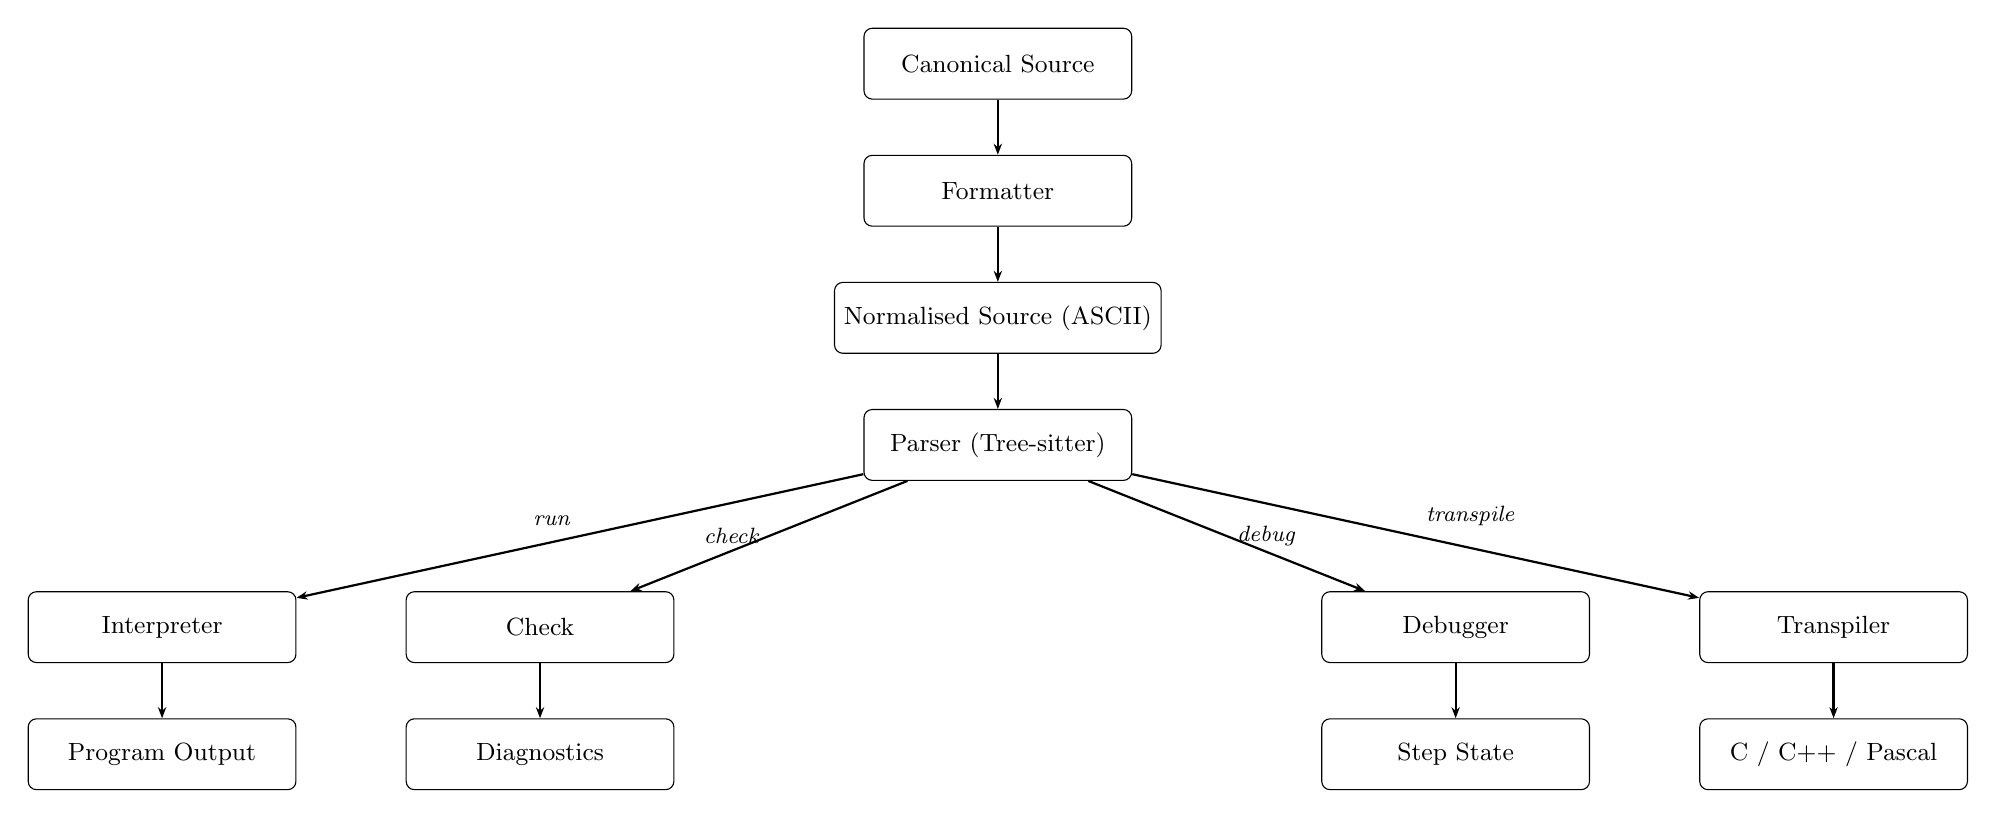
\begin{tikzpicture}[
  node distance  = 7mm and 22mm,
  box/.style     = {draw, rounded corners=3pt, minimum width=34mm,
                    minimum height=9mm, align=center, font=\small},
  arr/.style     = {-{Stealth[length=4pt]}, thick},
  lbl/.style     = {font=\footnotesize\itshape},
]
  \node[box] (src)   {Canonical Source};
  \node[box, below=of src]   (fmt)   {Formatter};
  \node[box, below=of fmt]   (ascii) {Normalised Source (ASCII)};
  \node[box, below=of ascii] (parse) {Parser (Tree-sitter)};

  \node[box, below left =14mm and 72mm of parse] (interp) {Interpreter};
  \node[box, below left =14mm and 24mm of parse] (linter) {Check};
  \node[box, below right=14mm and 24mm of parse] (debug)  {Debugger};
  \node[box, below right=14mm and 72mm of parse] (trans)  {Transpiler};

  \node[box, below=of interp] (out1) {Program Output};
  \node[box, below=of linter] (out2) {Diagnostics};
  \node[box, below=of debug]  (out3) {Step State};
  \node[box, below=of trans]  (out4) {C / C++ / Pascal};

  \draw[arr] (src)   -- (fmt);
  \draw[arr] (fmt)   -- (ascii);
  \draw[arr] (ascii) -- (parse);
  \draw[arr] (parse) -- node[lbl, above left  ]{run}       (interp);
  \draw[arr] (parse) -- node[lbl, left        ]{check}     (linter);
  \draw[arr] (parse) -- node[lbl, right       ]{debug}     (debug);
  \draw[arr] (parse) -- node[lbl, above right ]{transpile} (trans);
  \draw[arr] (interp) -- (out1);
  \draw[arr] (linter) -- (out2);
  \draw[arr] (debug)  -- (out3);
  \draw[arr] (trans)  -- (out4);
\end{tikzpicture}%
}
\caption{The Pseudo++ processing pipeline.  After normalisation and parsing, the
CST is handed to the interpreter, static analyser, debugger, or transpiler depending on the
requested operation.}
\label{fig:pipeline}
\end{figure}

% ─────────────────────────────────────────────────────────────────────────────
\section{Equivalence of Repetitive Control Structures}
\label{sec:loop-equivalence}

\subsection{Structured Programming and the Böhm-Jacopini Theorem}

The theoretical basis for loop equivalence lies in \textit{structured programming
theory}.  Böhm and Jacopini proved in 1966 \cite{bohm-jacopini} that any computable
function can be expressed using only three control-flow primitives: sequence,
selection (\texttt{if}), and a single repetition construct.  This result, together
with Dijkstra's influential argument against unstructured jumps \cite{dijkstra1968goto},
established the primacy of structured loops in procedural programming.
A practical consequence is that the four loop forms commonly found in procedural
languages --- \textit{for}, \textit{while}, \textit{do-while}, and
\textit{repeat-until} --- are mutually interconvertible: any loop can be rewritten using any other form, at the
cost of at most a guard condition or an unrolled first iteration.

This is not merely an academic curiosity.  The Romanian high-school computer science
curriculum explicitly teaches all four loop forms and expects students to
identify and apply these transformations in examination problems.
Providing an automated, interactive converter therefore has direct pedagogical value.

\subsection{Semantics of the Four Loop Forms}

Let $B$ denote the loop body (a finite sequence of statements), $C$ a Boolean
condition, $i$ a counter variable, $a$ the initial value, $b$ the bound, and $s > 0$
the step size.  The four loops have the following denotational semantics:

\begin{itemize}
  \item \textbf{for}: execute $B$ for $i = a,\, a{+}s,\, \ldots$ while $i \leq b$;
        zero or more iterations.
  \item \textbf{while}: while $C$, execute $B$; zero or more iterations.
  \item \textbf{do-while}: execute $B$, then repeat while $C$; at least one
        iteration.
  \item \textbf{repeat-until}: execute $B$, then repeat until $C$
        (i.e.\ while $\neg C$); at least one iteration.
\end{itemize}

The key structural distinction is between \textit{pre-test} loops (\textit{while},
\textit{for}) that may execute zero times, and \textit{post-test} loops
(\textit{do-while}, \textit{repeat-until}) that always execute at least once.
Crossing the boundary between the two families requires a guard.

\subsection{Transformation Rules}

The following semantics-preserving rewrite rules hold unconditionally:

\paragraph{while $\to$ do-while (and back).}
\[
  \textbf{while } C \;\textbf{do}\; B
  \;\;\equiv\;\;
  \textbf{if } C \;\textbf{then}\; (\textbf{do}\; B \;\textbf{while}\; C)
\]
\[
  \textbf{do}\; B \;\textbf{while}\; C
  \;\;\equiv\;\;
  B\,;\;\textbf{while } C \;\textbf{do}\; B
\]

\paragraph{for $\to$ while.}
\[
  \textbf{for}\; i \leftarrow a,\, b,\, s \;\textbf{do}\; B
  \;\;\equiv\;\;
  i \leftarrow a\,;\;\textbf{while}\; i \leq b \;\textbf{do}\; (B\,;\;i \leftarrow i + s)
\]

\paragraph{repeat-until $\to$ while (and back).}
\[
  \textbf{repeat}\; B \;\textbf{until}\; C
  \;\;\equiv\;\;
  B\,;\;\textbf{while}\; \neg C \;\textbf{do}\; B
\]

By composing these four base rules, all twelve directed pairwise conversions among
the four loop forms can be derived.  Pseudo++'s \texttt{equivalence} module
implements each conversion as a text-level rewrite over the CST, preserving the
original source indentation.

% ─────────────────────────────────────────────────────────────────────────────
\section{WebAssembly}
\label{sec:webassembly}

\subsection{Overview}

WebAssembly (Wasm) \cite{haas2017wasm,wasm-spec} is a binary instruction
format for a stack-based virtual machine, standardised by the W3C in 2019.  Its design goals are
portability, safety, and near-native execution speed in the browser.  A WebAssembly
module is a self-contained binary (\texttt{.wasm}) that exports and imports named
functions; the host (typically a JavaScript runtime) provides imports and calls
exports.

Key properties of the Wasm execution model:

\begin{itemize}
  \item \textbf{Linear memory}: a contiguous, byte-addressable memory region whose
        size is a multiple of 64~KiB.  The C heap and stack both reside in linear
        memory; pointer arithmetic is valid within this region.

  \item \textbf{Type safety}: all instructions are typed; the validator rejects
        ill-typed modules before execution.

  \item \textbf{Sandboxing}: a Wasm module cannot access host memory outside its
        own linear memory or perform arbitrary I/O; all interaction with the outside
        world happens through explicitly imported functions.

  \item \textbf{Determinism}: aside from NaN bit-patterns, Wasm execution is fully
        deterministic.
\end{itemize}

\subsection{Emscripten}

Emscripten \cite{emscripten} is an LLVM-based compiler toolchain that compiles C
and C++ to WebAssembly together with a JavaScript glue layer.  Given a C source
file, Emscripten compiles it to LLVM IR via \texttt{clang}, lowers it to Wasm
via \texttt{wasm-ld} and \texttt{wasm-opt}, and generates a JavaScript companion
(\texttt{.js}) that instantiates the module, provides standard C library shims,
and exposes exported C functions to JavaScript callers.

Functions to be exported must be annotated with \texttt{EMSCRIPTEN\_KEEPALIVE}
to prevent dead-code elimination, or listed via the
\texttt{-sEXPORTED\_FUNCTIONS} linker flag.


% ─────────────────────────────────────────────────────────────────────────────
\section{Statement-Level Step-Through Debugging}
\label{sec:debugging}

\subsection{Interactive Debugging in Educational Contexts}

Step-through debugging allows a student to observe a program's behaviour one
statement at a time, inspecting variable values and control flow at each point.
This is particularly valuable when learning programming: rather than reading static
code, the student sees the program \textit{in motion} --- which variable changes,
which branch is taken, how a loop counter evolves \cite{wing2006ct}.
More advanced tools support stepping \emph{backwards} through execution history
(omniscient or reversible debugging \cite{lewis2003omniscient,reversible-debugging});
Pseudo++ provides forward-only stepping.

Pseudo++'s debugger exposes two user-facing operations:

\begin{itemize}
  \item \textbf{Step Into} (one statement at a time): executes the next statement,
        highlights the corresponding source line in the editor, and updates the
        variable inspection panel.
  \item \textbf{Continue} (run to completion): resumes fast execution without
        step-by-step visibility, stopping only when the program finishes, encounters
        a runtime error, or needs user input.
\end{itemize}


\chapter{The Pseudo++ Toolchain}
\label{chap:implementation}

This chapter describes the design and implementation of the Pseudo++ toolchain,
a complete software pipeline for writing, executing, debugging, and transpiling
Romanian-style pseudocode as taught at the Romanian high-school level.
The toolchain is written in C (core library) and JavaScript (web editor,
Tree-sitter grammar), and is distributed as a native command-line binary
and a browser-based editor that comes bundled with the core implementation
compiled to WebAssembly.

% ─────────────────────────────────────────────────────────────────────────────
\section{System Architecture}
\label{sec:architecture}

The Pseudo++ toolchain is structured as four layers of independent modules,
each with a narrow public interface. Figure~\ref{fig:modules} shows the
compile-time dependency graph of all modules grouped by layer.

\begin{figure}[h]
\centering
\resizebox{0.85\linewidth}{!}{%
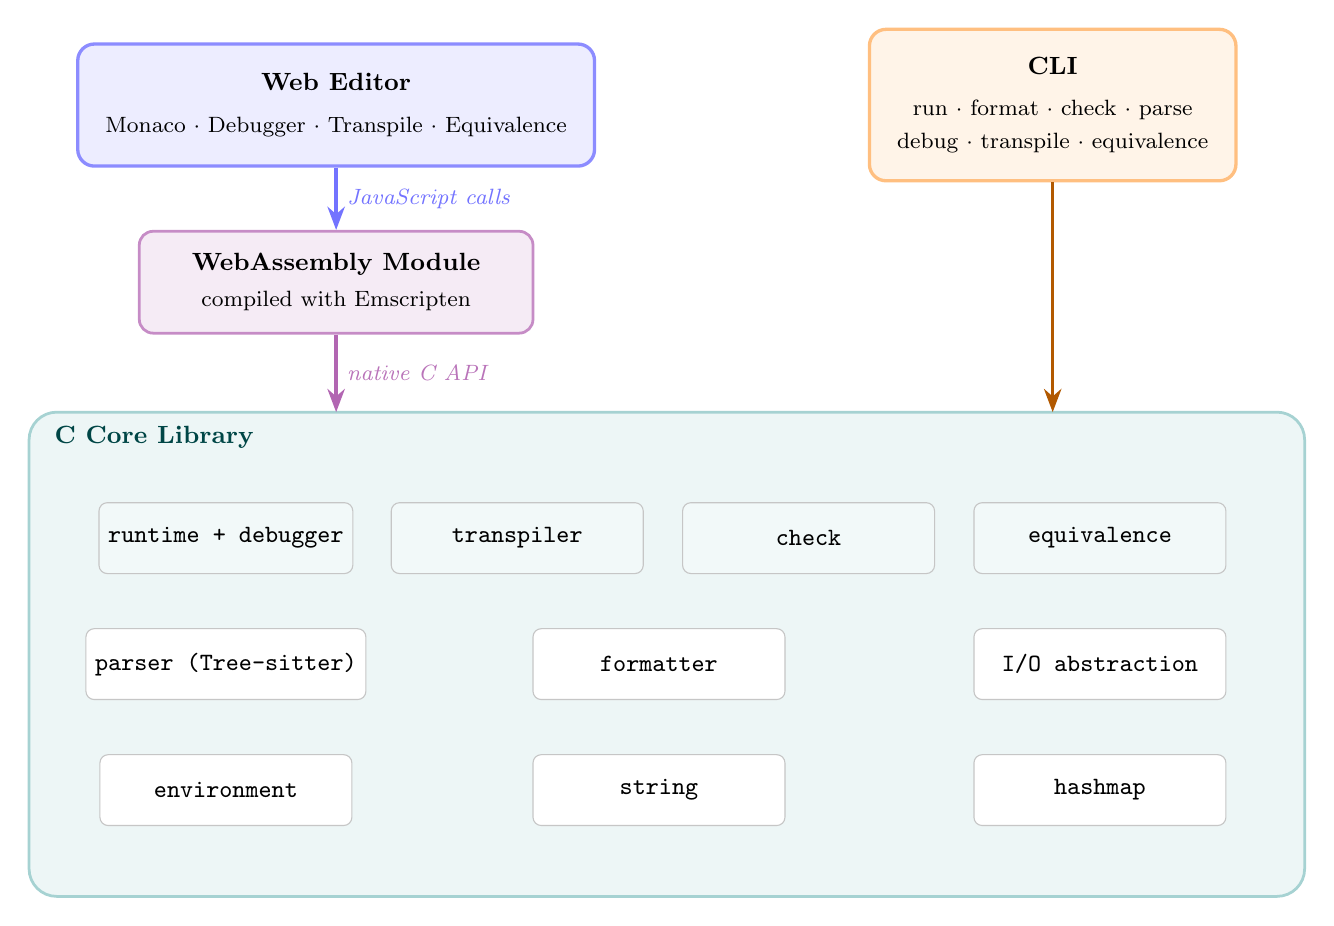
\begin{tikzpicture}[
    product/.style = {
        draw, line width=1.2pt, rounded corners=6pt,
        font=\small, align=center, inner sep=10pt
    },
    build/.style = {
        draw, line width=1pt, rounded corners=5pt,
        font=\small, align=center, inner sep=8pt
    },
    cmod/.style = {
        draw=gray!45, rounded corners=3pt,
        minimum width=3.2cm, minimum height=0.9cm,
        font=\small\ttfamily, align=center, fill=white
    },
    arr/.style = {-Stealth, line width=1.2pt},
]

%% ── C Core Library ──────────────────────────────────────────────────────
\begin{pgfonlayer}{background}
  \fill[teal!7, rounded corners=10pt]
    (-1.0,-0.65) rectangle (15.2, 5.5);
  \draw[teal!35, line width=1pt, rounded corners=10pt]
    (-1.0,-0.65) rectangle (15.2, 5.5);
\end{pgfonlayer}
\node[font=\small\bfseries\color{teal!55!black}, anchor=north west]
  at (-0.8, 5.45) {C Core Library};

%% Capabilities row (y = 3.9)  — teal tint marks the top layer
\node[cmod, fill=teal!5] (rt) at (1.5,  3.9) {runtime + debugger};
\node[cmod, fill=teal!5] (tr) at (5.2,  3.9) {transpiler};
\node[cmod, fill=teal!5] (chk) at (8.9, 3.9) {check};
\node[cmod, fill=teal!5] (eq) at (12.6, 3.9) {equivalence};

%% Foundation row (y = 2.3)
\node[cmod] (parse) at (1.5,  2.3) {parser (Tree-sitter)};
\node[cmod] (lint)  at (7.0,  2.3) {formatter};
\node[cmod] (io)    at (12.6, 2.3) {I/O abstraction};

%% Utilities row (y = 0.7)
\node[cmod] (env)  at (1.5,  0.7) {environment};
\node[cmod] (str)  at (7.0,  0.7) {string};
\node[cmod] (hmap) at (12.6, 0.7) {hashmap};

%% ── WebAssembly build ────────────────────────────────────────────────
\node[build, fill=violet!8, draw=violet!45,
      minimum width=5.0cm, minimum height=1.0cm]
  (wasm) at (2.9, 7.15)
  {{\bfseries WebAssembly Module}\\[2pt]
   {\footnotesize compiled with Emscripten}};

%% ── Products ─────────────────────────────────────────────────────────
\node[product, fill=blue!7, draw=blue!45,
      minimum width=5.2cm, minimum height=1.55cm]
  (web) at (2.9, 9.4)
  {{\bfseries Web Editor}\\[4pt]
   {\footnotesize Monaco $\cdot$ Debugger $\cdot$ Transpile $\cdot$ Equivalence}};

\node[product, fill=orange!9, draw=orange!50,
      minimum width=4.4cm, minimum height=1.55cm]
  (cli) at (12.0, 9.4)
  {{\bfseries CLI}\\[4pt]
   {\footnotesize run $\cdot$ format $\cdot$ check $\cdot$ parse}\\[1pt]
   {\footnotesize debug $\cdot$ transpile $\cdot$ equivalence}};

%% ── Arrows ───────────────────────────────────────────────────────────
\draw[arr, blue!55]
  (web.south) -- node[right, font=\footnotesize\itshape, text=blue!55]
  {JavaScript calls} (wasm.north);

\draw[arr, violet!60]
  (wasm.south) -- node[right, font=\footnotesize\itshape, text=violet!55]
  {native C API} (2.9, 5.5);

\draw[arr, orange!70!black]
  (cli.south) -- (12.0, 5.5);

\end{tikzpicture}%
}
\caption{Compile-time dependency graph of the Pseudo++ modules, grouped by layer.
  The C core library (teal) is compiled to both a native CLI binary and a WebAssembly
  module loaded by the web editor.}
\label{fig:modules}
\end{figure}

The modules and their responsibilities are:

\begin{description}
  \item[\texttt{formatter}] Normalises the raw source text before parsing: it
        replaces Unicode mathematical symbols (e.g.\ $\leq$, $\neq$) with
        their ASCII equivalents and re-indents the code structurally.

  \item[\texttt{check}] Performs static semantic analysis on the CST after
        parsing, reporting diagnostics (errors and warnings with codes such as
        \texttt{W001}) for issues like unused variables or suspicious patterns.

  \item[\texttt{parser}] Wraps the Tree-sitter incremental parser with the
        custom \texttt{pseudo} grammar, exposes the resulting concrete syntax
        tree (CST), and provides helper utilities for navigating and extracting
        text from CST nodes.

  \item[\texttt{runtime}] Implements the tree-walking interpreter.  It
        subdivides into three sub-modules: \texttt{value} (runtime values and
        arithmetic), \texttt{environment} (variable store), and
        \texttt{interpreter} (execution engine with explicit stack).

  \item[\texttt{debugger}] Extends the interpreter with variable inspection
        and JSON serialisation of runtime state for the browser front end.

  \item[\texttt{transpiler}] Converts the CST to equivalent C, C++, or Pascal
        source, performing a two-pass analysis: first collecting variable types,
        then emitting the target code.

  \item[\texttt{equivalence}] Implements loop-equivalence transformations,
        converting a loop construct of one kind (e.g.\ \texttt{for}) into any
        of the other three (\texttt{while}, \texttt{do\_while}, \texttt{repeat})
        while preserving semantics.

  \item[\texttt{io}] Provides an abstract I/O interface with two concrete
        backends: \texttt{io\_stdio} for the CLI and \texttt{io\_buffered} for
        the WebAssembly build.

  \item[\texttt{wasm}] An Emscripten bridge that exports the runtime,
        transpiler, and equivalence module as \texttt{EMSCRIPTEN\_KEEPALIVE}
        C functions callable from JavaScript.

  \item[\texttt{cli}] The command-line entry point, supporting \texttt{run},
        \texttt{format}, \texttt{check}, \texttt{parse}, \texttt{debug},
        \texttt{transpile}, and \texttt{equivalence} sub-commands.
\end{description}

% ─────────────────────────────────────────────────────────────────────────────
\section{Language Grammar}
\label{sec:grammar}

The grammar for the Pseudo++ language is specified as a Tree-sitter
\cite{treesitter} grammar in JavaScript (\texttt{grammar.js}).  It defines
the notation established by convention in Romanian high-school CS textbooks
and baccalaureate examination papers \cite{romanian-curriculum}.

\subsection{Statement Forms}

The top-level production \texttt{program} is a repetition of \texttt{stmt}
nodes.  Each statement is one of:

\begin{itemize}
  \item \textbf{Assignment} (\texttt{assign}):
        \texttt{x <- expr} --- assigns the value of \textit{expr} to variable
        \texttt{x}.
  \item \textbf{Swap} (\texttt{swap}):
        \texttt{x <-> y} --- exchanges the values of \texttt{x} and \texttt{y}.
  \item \textbf{Read} (\texttt{read}):
        \texttt{citeste x, y, z} --- reads values from standard input.
  \item \textbf{Write} (\texttt{write}):
        \texttt{scrie expr1, expr2} --- writes values to standard output.
  \item \textbf{Conditional} (\texttt{if}):
        \texttt{daca} \textit{cond} \texttt{atunci} \ldots\
        [\texttt{altfel} \ldots] \texttt{sf}.
  \item \textbf{Counting loop} (\texttt{for}):
        \texttt{pentru i <- start, end[, step] executa} \ldots\ \texttt{sf}.
  \item \textbf{Pre-condition loop} (\texttt{while}):
        \texttt{cat timp} \textit{cond} \texttt{executa} \ldots\ \texttt{sf}.
  \item \textbf{Post-condition loop} (\texttt{do\_while}):
        \texttt{executa} \ldots\ \texttt{cat timp} \textit{cond}.
  \item \textbf{Repeat-until loop} (\texttt{repeat}):
        \texttt{repeta} \ldots\ \texttt{pana cand} \textit{cond}.
  \item \textbf{Compound statement} (\texttt{multi\_stmt}): two or more simple
        statements separated by semicolons, used where only a single statement
        is syntactically permitted.
\end{itemize}

\subsection{Expression Hierarchy}

Expressions follow a standard precedence hierarchy encoded via Tree-sitter's
\texttt{prec.left} operator:

\begin{center}
\begin{tabular}{c l l}
\hline
\textbf{Level} & \textbf{Operator(s)} & \textbf{Node type} \\
\hline
1 (lowest) & \texttt{SAU / sau}                        & \texttt{or\_expr} \\
2          & \texttt{SI / si}                           & \texttt{and\_expr} \\
3          & \texttt{NOT / not}                         & \texttt{not\_expr} \\
4          & \texttt{= != < <= > >=}                    & \texttt{compare\_expr} \\
5          & \texttt{+ -}                               & \texttt{add\_expr} \\
6          & \texttt{* / \%}                            & \texttt{mul\_expr} \\
7 (highest)& \texttt{-(x)}, \texttt{[x]}, $\sqrt{x}$ & \texttt{neg\_expr}, \texttt{floor}, \texttt{sqrt\_expr} \\
\hline
\end{tabular}
\end{center}

Atoms (\texttt{atom}) are integer literals, floating-point literals, string
literals, or identifiers.  Parenthesised sub-expressions (\texttt{paren}) reset
precedence.  The floor operator uses bracket notation (\texttt{[expr]}), which
maps to integer truncation, while the square-root operator uses the radical
symbol ($\sqrt{\phantom{x}}$).

% ─────────────────────────────────────────────────────────────────────────────
\section{Source Normalisation}
\label{sec:formatter}

The Romanian high-school pseudocode notation, established by convention
through textbooks and baccalaureate examination papers \cite{romanian-curriculum},
uses a rich set
of Unicode characters: relational symbols ($\leq$, $\neq$, $\geq$), assignment and
swap arrows ($\leftarrow$, $\leftrightarrow$), box-drawing characters for
structural indentation (box-drawing bar), a filled square ($\blacksquare$) as the
block-closing symbol instead of the keyword \texttt{sf}, and letters with
Romanian diacritics.  This notation is the \emph{canonical} form of the
language --- it is not incidental variation but the deliberate typographic
standard taught in schools.

Formalising this notation directly into a parser grammar would tightly couple
the grammar to a specific Unicode encoding and make the language impractical to
type in a plain-text environment.  The toolchain therefore introduces a
deliberate split: the \emph{source language} that users write (and that the
parser accepts) uses ASCII-compatible tokens, while the \emph{display language}
visible in the web editor renders those tokens back into the canonical Unicode
form via ligatures and glyph substitutions.  This rendering is purely visual
and optional: a toggle button in the editor enables or disables it, leaving
the underlying source file unchanged in either case.

The formatter is the bridge between the two representations.  It accepts source in
either form --- canonical Unicode or ASCII --- and produces the normalised ASCII
form consumed by the parser.  The normalisation pipeline consists of two passes:

\paragraph{Pass 1 --- Symbol Substitution.}
The formatter maintains a static hash map that maps Unicode byte sequences to their
ASCII equivalents (Table~\ref{tab:substitutions}).  The pass iterates through
the source byte-by-byte, scanning the substitution map at each position for the
longest matching key (a greedy, maximum-munch strategy).  When a match is found
the corresponding replacement string is appended to the output and the cursor
advances by the match length; otherwise the current byte is copied verbatim.

\begin{table}[h]
\centering
\small
\begin{tabular}{l l l}
\hline
\textbf{Canonical input} & \textbf{Category} & \textbf{ASCII output} \\
\hline
$\leq$, $\neq$, $\geq$        & Relational symbols   & \texttt{<=}, \texttt{!=}, \texttt{>=} \\
$\leftarrow$                   & Assignment arrow     & \texttt{<-} \\
$\leftrightarrow$              & Swap arrow           & \texttt{<->} \\
$\blacksquare$ (U+25A0)        & Block-close square   & \texttt{sf} \\
box-drawing bar (U+2502)       & Structural indent    & 4 spaces \\
\texttt{\textquotedblleft}, \texttt{\quotedblbase} & Curly quotes & \texttt{"} \\
\textit{ă}, \textit{â}, \textit{î}, \textit{ș}, \textit{ț} & Romanian diacritics & \texttt{a}, \texttt{a}, \texttt{i}, \texttt{s}, \texttt{t} \\
\hline
\end{tabular}
\caption{Selected substitution rules applied by the formatter in Pass 1.
  The canonical Unicode notation is the standard form used in Romanian
  high-school textbooks and exam papers; the ASCII output is the form
  accepted by the Tree-sitter grammar.}
\label{tab:substitutions}
\end{table}

\paragraph{Pass 2 --- Structural Re-indentation.}
After symbol substitution the source may have inconsistent indentation,
particularly when the box-drawing indentation markers have been replaced by
spaces.  The second pass strips all leading whitespace from every line and
recomputes indentation from scratch based on a set of \emph{indent triggers}:

\begin{itemize}
  \item \textit{Indent-after} lines --- lines whose last word is \texttt{atunci},
        \texttt{executa}, \texttt{altfel}, or whose first word is \texttt{repeta}
        --- increase the indentation level for the next line.
  \item \textit{Dedent-before} lines --- \texttt{sf} alone, \texttt{altfel} as
        the first word, and the closing \texttt{pana cand} of a repeat loop ---
        decrease the indentation level before the line is emitted.
\end{itemize}

The result is a clean, consistently-indented ASCII source that the Tree-sitter
parser can analyse reliably.

% ─────────────────────────────────────────────────────────────────────────────
\section{Parsing and CST Construction}
\label{sec:parsing-ast}

The \texttt{parser} module wraps the Tree-sitter C API.  Its public interface
centres on an opaque \texttt{parser\_t} struct that owns a
\texttt{TSParser} (the Tree-sitter parser instance), a \texttt{TSTree} (the
last parse result), and a copy of the normalised source string.

\paragraph{Parsing.}
\texttt{parser\_parse()} first copies the source, then calls
\texttt{ts\_parser\_parse\_string()}.  Tree-sitter guarantees a result tree
even on malformed input, using \texttt{ERROR} and \texttt{MISSING} synthetic
nodes to indicate problem sites.  After the C API call, the function performs a
depth-first walk of the resulting tree looking for the first such error node;
if one is found, it reports the row and column of the error and constructs a
human-readable diagnostic message.

\paragraph{Node Helpers.}
Because the interpreter and transpiler perform extensive tree traversal,
\texttt{parser.c} also provides a set of helper functions used throughout the
codebase:

\begin{itemize}
  \item \texttt{parser\_node\_is\_type(node, type)} --- string-compares the
        node's grammar type against a constant.
  \item \texttt{parser\_child\_by\_field(node, field)} --- wraps
        \texttt{ts\_node\_child\_by\_field\_name}, used to retrieve named
        children such as \texttt{condition}, \texttt{left}, \texttt{right},
        \texttt{var}, \texttt{start}, \texttt{end}, and \texttt{step}.
  \item \texttt{parser\_node\_text(parser, node)} --- extracts the source
        substring corresponding to a node by using its start and end byte
        offsets.
  \item \texttt{parser\_pretty\_tree()} / \texttt{parser\_debug\_tree()} ---
        produce human-readable renderings of the CST for diagnostic purposes.
\end{itemize}

% ─────────────────────────────────────────────────────────────────────────────
\section{Interpreter}
\label{sec:interpreter}

\subsection{Value Representation}
\label{subsec:values}

Runtime values are represented by a heap-allocated, tagged-union type
\texttt{value\_t}:

\begin{lstlisting}[language=C, basicstyle=\ttfamily\small]
struct value {
    value_type_t type;        /* VALUE_INT | VALUE_FLOAT | VALUE_STRING */
    union {
        int64_t   int_val;
        double    float_val;
        string_t* string_val;
    };
};
\end{lstlisting}

\noindent
The three types cover the full range of values expressible in Romanian
baccalaureate pseudocode.  The following design decisions govern arithmetic:

\begin{itemize}
  \item \textbf{Type promotion.}  When one operand is \texttt{VALUE\_FLOAT}
        and the other is \texttt{VALUE\_INT}, the integer is promoted via
        \texttt{value\_to\_float()} before the operation is applied.
  \item \textbf{Division always yields a float.}
        The \texttt{/} operator always returns a \texttt{double}, mirroring
        the mathematical convention used in Romanian textbooks.  Integer
        division is expressed explicitly with the floor operator \texttt{[a/b]}.
  \item \textbf{Modulo operates on integers.}
        The \texttt{\%} operator truncates both operands to \texttt{int64\_t}
        before computing the remainder.
  \item \textbf{Square root returns an integer when the result is exact.}
        If \texttt{sqrt(d) == floor(sqrt(d))}, the result is returned as
        \texttt{VALUE\_INT}.
  \item \textbf{String concatenation.}
        The \texttt{+} operator is overloaded: when both operands are strings
        it performs concatenation; mixed string/numeric operands are a
        type error.
\end{itemize}

Logical operations (\texttt{SI}, \texttt{SAU}, \texttt{NOT}) operate on the
\emph{truthiness} of any value: a numeric zero and an empty string are false;
everything else is true.  They always return \texttt{VALUE\_INT} (1 or 0).

All arithmetic functions follow the same error-reporting convention: an
optional \texttt{value\_error\_t* err} output parameter is set to
\texttt{VALUE\_OK}, \texttt{VALUE\_ERR\_TYPE}, \texttt{VALUE\_ERR\_DIV\_ZERO},
or \texttt{VALUE\_ERR\_NEGATIVE\_SQRT}.

\subsection{Execution Environment}
\label{subsec:environment}

Variables are stored in a flat \texttt{environment\_t}, implemented as an
open-addressing hash table with linear probing.  The table uses three slot
states (\texttt{SLOT\_EMPTY}, \texttt{SLOT\_OCCUPIED}, \texttt{SLOT\_DELETED})
to support deletion without disrupting existing probe chains.  The FNV-1a hash
function \cite{fnv-hash} is used for string keys:

\begin{lstlisting}[language=C, basicstyle=\ttfamily\small]
static uint64_t hash_string(const char* str) {
    uint64_t hash = 14695981039346656037ULL;
    while (*str) {
        hash ^= (uint64_t)(unsigned char)(*str++);
        hash *= 1099511628211ULL;
    }
    return hash;
}
\end{lstlisting}

The table starts with capacity 16.  When the combined occupancy of
\texttt{OCCUPIED} and \texttt{DELETED} slots exceeds a 70\,\% load factor,
\texttt{env\_resize()} doubles the capacity and rehashes all live entries.
Ownership of values is transferred on set: the table takes ownership of
the \texttt{value\_t*} passed to \texttt{env\_set()}, and the previous value
(if any) is destroyed in place.

An important semantic detail is that Pseudo++ variables are \emph{implicitly
initialised}: reading an undeclared variable returns an integer zero and also
creates the binding, matching the convention in Romanian textbook examples
where variables are used before being formally assigned.

\subsection{Expression Evaluation}
\label{subsec:expressions}

Expressions are evaluated by a recursive \texttt{eval\_expr()} function that
walks the CST nodes produced by Tree-sitter.  For binary operators
(\texttt{add\_expr}, \texttt{mul\_expr}, \texttt{compare\_expr}) the function
extracts the named children \texttt{left}, \texttt{op}, and \texttt{right},
evaluates the sub-expressions recursively, reads the operator text, and
dispatches to the appropriate \texttt{value\_*} arithmetic function.

Short-circuit evaluation is implemented for the logical connectives:
\texttt{or\_expr} returns 1 immediately if the left operand is truthy without
evaluating the right; \texttt{and\_expr} returns 0 immediately if the left
operand is falsy.

After each binary expression evaluation the runtime checks whether an error
flag was set; if so, it transitions to the \texttt{EXEC\_ERROR} state and
stores the error message, halting further execution.

\subsection{Control Flow}
\label{subsec:control-flow}

The interpreter uses an \emph{explicit execution stack} rather than recursion.
This design choice serves two goals: it prevents stack overflow for deeply
nested pseudocode, and it allows the debugger to capture and restore the full
execution state as a data structure.

The stack holds up to \texttt{MAX\_STACK\_DEPTH} frames.  Each frame
(\texttt{exec\_frame\_t}) records:

\begin{itemize}
  \item the \texttt{frame\_type\_t} (one of
        \texttt{FRAME\_PROGRAM}, \texttt{FRAME\_BLOCK}, \texttt{FRAME\_IF},
        \texttt{FRAME\_FOR}, \texttt{FRAME\_WHILE}, \texttt{FRAME\_DO\_WHILE},
        \texttt{FRAME\_REPEAT});
  \item the corresponding CST node;
  \item a \texttt{phase} integer and \texttt{child\_idx} counter tracking
        which part of the construct has already been executed;
  \item loop-specific fields (\texttt{loop\_current}, \texttt{loop\_end},
        \texttt{loop\_step}, \texttt{loop\_var}) for the \texttt{for} frame.
\end{itemize}

A compile-time dispatch table maps each frame type to its step function:

\begin{lstlisting}[language=C, basicstyle=\ttfamily\small]
static const frame_step_fn k_step_fns[] = {
    [FRAME_PROGRAM]  = step_program,
    [FRAME_IF]       = step_if,
    [FRAME_FOR]      = step_for,
    [FRAME_WHILE]    = step_while,
    [FRAME_DO_WHILE] = step_do_while,
    [FRAME_REPEAT]   = step_repeat,
    [FRAME_BLOCK]    = step_block,
};
\end{lstlisting}

Each step function advances the frame by one \emph{phase} and returns a
Boolean indicating whether a \emph{visible action} occurred.  Visible actions
include executing a simple statement, evaluating a loop condition, and
terminating the program; invisible actions are internal transitions such as
resetting \texttt{child\_idx} at the start of a new loop iteration.

The public API exposes two execution modes:

\begin{itemize}
  \item \texttt{runtime\_step()} --- advances to the next visible action.
        Used by the step-by-step debugger.
  \item \texttt{runtime\_run()} --- runs to completion or the next input
        request via a tight loop with no overhead.  Used by both the CLI
        \texttt{run} command and the web editor's Run button.
\end{itemize}

The \texttt{EXEC\_NEEDS\_INPUT} state suspends execution when a \texttt{read}
statement encounters an unavailable token.  The web front end supplies the
missing token through \texttt{io\_buffered} and calls \texttt{runtime\_resume()}
to continue.

% ─────────────────────────────────────────────────────────────────────────────
\section{Debugger}
\label{sec:debugger}

The debugger extends the interpreter with step-by-step execution and runtime
state inspection.  The web editor exposes two operations:
\textbf{Step Into} (advance one visible action) and \textbf{Continue} (run to
completion or the next input request).  After each step, the front end displays
the currently executing line, the full variable table, and --- when the step
involved evaluating a condition --- the condition text and its boolean result.

\paragraph{State serialisation.}
The function \texttt{runtime\_get\_variables\_json()} serialises the current
variable table to a JSON array of \texttt{\{name, value, type\}} objects, with
proper JSON string escaping.  This JSON string is the primary mechanism by
which the WebAssembly runtime communicates variable state to the JavaScript
front end on each step.

The WASM bridge combines the variable table, the current line number, the
execution status, and optional condition information into a single JSON
response per step via \texttt{pseudo\_debug\_step()}.

\paragraph{Condition visualisation.}
When the statement about to execute is a conditional or loop guard, the runtime
additionally captures the condition expression text and its boolean result in a
\texttt{condition\_info\_t} struct stored on the runtime object.  The bridge
layer serialises this alongside the variable state, letting the student see not
only \textit{which} branch was taken but \textit{why} --- the exact condition
text and its evaluated truth value at that step.

% ─────────────────────────────────────────────────────────────────────────────
\section{Transpiler}
\label{sec:transpiler}

\subsection{Code Generation for C, C++, and Pascal}
\label{subsec:codegen}

The transpiler converts a normalised Pseudo++ CST to compilable source code in
C, C++, or Pascal.  Because these three languages differ in significant ways ---
type declarations, operator syntax, string literals, and logical keyword
precedence --- the transpiler abstracts all language-specific choices into a
\texttt{lang\_ops\_t} record populated once at construction time:

\begin{lstlisting}[language=C, basicstyle=\ttfamily\small]
typedef struct {
    const char* assign_op;   /* "=" (C/C++) or ":=" (Pascal) */
    const char* eq_op;       /* "==" or "="  */
    const char* ne_op;       /* "!=" or "<>" */
    const char* or_op;       /* "||" or "or" */
    const char* and_op;      /* "&&" or "and"*/
    const char* not_kw;      /* "!"  or "not " */
    const char* floor_open;  /* "(int)(" or "trunc(" */
    const char* floor_close; /* ")" */
    bool is_pascal;
    bool is_cpp;
} lang_ops_t;
\end{lstlisting}

Transpilation proceeds in two passes:

\paragraph{Pass 1 --- Variable Type Collection.}
\texttt{collect\_vars()} performs a depth-first walk of the CST.  For each
assignment or read statement it records the inferred type of the target
variable in a hash map (\texttt{var\_types}).  The inference rules are:

\begin{itemize}
  \item If the right-hand-side expression contains a string literal, the
        variable is typed as \texttt{string}.
  \item If it contains a floating-point literal (a number with a decimal
        point), it is typed as \texttt{double}.
  \item Otherwise it is typed as \texttt{int}.
\end{itemize}

The first assignment wins for the purpose of code generation; subsequent
assignments may change the value but not the declared type in the target
language.  This is a transpiler-level heuristic, not a language restriction:
the interpreter is fully dynamically typed and allows a variable to hold
values of different types at different points in execution.

\paragraph{Pass 2 --- Code Emission.}
The emission pass walks the CST recursively via \texttt{gen\_stmt()}, using
the \texttt{lang\_ops\_t} record to emit the correct syntax for each construct.
Several language-specific concerns deserve mention:

\begin{itemize}
  \item \textbf{C variable declarations.}  C requires variables to be declared
        before use.  Rather than adding a separate declaration section, the
        transpiler hoists declarations \emph{inline}: the helper
        \texttt{hoist\_vars()} scans each block before emitting its first
        statement and pre-declares any variable first assigned or read in that
        block.  A \texttt{declared\_vars} hash map prevents duplicate
        declarations.  C strings are emitted as \texttt{char name[256]};
        C++ strings use \texttt{std::string}.

  \item \textbf{Pascal variable section.}  For Pascal, variable declarations
        are collected globally during Pass 1 and emitted in a \texttt{var}
        block at the top of the program before the \texttt{begin} keyword.

  \item \textbf{Pascal logical operator precedence.}  In Pascal, \texttt{and}
        and \texttt{or} bind \emph{more tightly} than comparison operators,
        unlike C where \texttt{\&\&} and \texttt{||} bind less tightly.
        To preserve semantics, the transpiler wraps each operand of an
        \texttt{and\_expr} or \texttt{or\_expr} in parentheses when targeting
        Pascal.

  \item \textbf{Pascal string literals.}  String literals are enclosed in
        single quotes in Pascal.  The transpiler re-encodes any embedded
        single quotes using Pascal's doubling convention (\texttt{''}).
\end{itemize}

\subsection{Loop Equivalence Transformations}
\label{subsec:loop-transforms}

The loop equivalence module implements a pedagogically important feature:
given any loop in a Pseudo++ program, it rewrites that loop into an
equivalent form using a different loop construct, grounded in the
interconvertibility established by Böhm and Jacopini \cite{bohm-jacopini}
and the structured programming principles of Dijkstra \cite{dijkstra1968goto}.
This allows students to practise the mechanical equivalence proofs required
at the baccalaureate exam.

The module accepts a source string, a 0-indexed target line identifying the
loop to transform, and the desired output construct (\texttt{FOR},
\texttt{WHILE}, \texttt{DO\_WHILE}, or \texttt{REPEAT}).  It then:

\begin{enumerate}
  \item Runs the source through the formatter and parser to obtain a CST.
  \item Locates the loop node at the specified line via DFS.
  \item Extracts the loop header fields (\texttt{var}, \texttt{start},
        \texttt{end}, \texttt{step}, \texttt{condition}) and body text from
        the CST and the raw source string.
  \item Constructs the target loop form by selecting the appropriate skeleton
        and filling in the extracted fields.
  \item Splices the new loop text back into the original source, preserving
        all preceding and following code unchanged.
\end{enumerate}

Indentation is preserved by detecting the loop's own indentation level from
the source and replicating it in the emitted loop.

% ─────────────────────────────────────────────────────────────────────────────
\section{I/O Abstraction and WebAssembly Integration}
\label{sec:wasm}

\subsection{I/O Abstraction}

The runtime communicates with the outside world exclusively through an abstract
\texttt{io\_t} interface:

\begin{lstlisting}[language=C, basicstyle=\ttfamily\small]
typedef struct {
    const char* (*read)(io_t*);   /* returns next token or NULL */
    void (*write)(io_t*, const char*);
    void (*destroy)(io_t*);
} io_ops_t;

struct io { io_ops_t ops; };
\end{lstlisting}

Two concrete implementations are provided:

\begin{itemize}
  \item \texttt{io\_stdio} --- delegates directly to \texttt{scanf} and
        \texttt{printf}, used by the CLI.
  \item \texttt{io\_buffered} --- maintains an input queue and an output
        queue.  JavaScript pushes input tokens by calling
        \texttt{pseudo\_push\_input()} (a WASM export) and pulls output by
        calling \texttt{pseudo\_pull\_output()}.  When the input queue is empty,
        \texttt{read()} returns \texttt{NULL}, causing the runtime to transition
        to \texttt{EXEC\_NEEDS\_INPUT}.
\end{itemize}

\subsection{WebAssembly Bridge}

The WASM build compiles the entire C library with Emscripten \cite{emscripten},
targeting the WebAssembly instruction format \cite{haas2017wasm}.  The bridge
module (\texttt{wasm/bridge.c}) instantiates a singleton \texttt{runtime\_t}
and a singleton \texttt{io\_buffered}, then exposes the toolchain to
JavaScript via \texttt{EMSCRIPTEN\_KEEPALIVE}-annotated functions, which are
exported by name from the resulting \texttt{.wasm} module.  The exported
surface includes functions for initialisation, source loading, single-step and
run-to-completion execution, input supply, output retrieval, variable
inspection, transpilation, and loop equivalence.

Separating the I/O layer behind an interface means that the \emph{same}
runtime and debugger C code is used in both the CLI and the browser --- only
the I/O backend differs.

% ─────────────────────────────────────────────────────────────────────────────
\section{Web Editor}
\label{sec:editor}

The web editor is a single-page application built around the Monaco Editor
\cite{monaco}, the same editing component that powers Visual Studio Code.
For the \texttt{pseudocode} language, the editor registers:

\begin{itemize}
  \item A \textbf{Monarch tokeniser} \cite{monarch} that classifies tokens
        into keyword, operator, string, number, comment, and identifier
        categories for syntax highlighting.
  \item A \textbf{language configuration} that specifies bracket pairs
        (for auto-closing), the line-comment token, and auto-indentation
        rules.
\end{itemize}

At runtime the JavaScript application loads the compiled WASM module and
communicates with it through the exported C functions.  The interface
provides:

\begin{itemize}
  \item \textbf{Run} --- compiles the editor content, sends it to the WASM
        runtime, and streams output tokens to the output pane.
  \item \textbf{Step / Step Over} --- calls the corresponding WASM step
        function (\texttt{pseudo\_debug\_step} or \texttt{pseudo\_step\_over}),
        which returns a JSON object containing the current line, variable table,
        execution status, and condition information; the front end uses this to
        update the highlighted line and the variable inspector panel.
  \item \textbf{Transpile} --- calls the WASM transpiler with the selected
        target language and displays the result in a read-only Monaco pane.
  \item \textbf{Loop Equivalence} --- identifies the loop under the cursor
        and passes it to the equivalence module.
\end{itemize}


\chapter{Evaluation}
\label{chap:evaluation}

\section{Testing Methodology}
\label{sec:methodology}

\section{Unit Testing}
\label{sec:unit-tests}

\section{Integration Testing on BAC Examination Subjects (2020--2025)}
\label{sec:bac-tests}

\subsection{Dataset Description}
\label{subsec:dataset}

\subsection{Results}
\label{subsec:results}

\section{Transpiler Correctness Verification}
\label{sec:transpiler-eval}

\section{Performance Analysis}
\label{sec:performance}

\section{Discussion}
\label{sec:discussion}

\chapter{Conclusions}
\label{chap:conclusions}

% ─────────────────────────────────────────────────────────────────────────────
\section{Summary}
\label{sec:summary}

This thesis presented Pseudo++, an open-source toolchain for the Romanian
baccalaureate pseudocode dialect.  The motivating gap was clear: despite
pseudocode being a central part of the Romanian high-school CS curriculum,
no complete execution environment existed for it.  Students had to
mentally trace programs by hand, with no automated way to verify whether
a solution was correct.

The toolchain addresses this gap through eight components built around a
single C core library: a Tree-sitter grammar that formally captures the
dialect's syntax, a source formatter that normalises Unicode notation to
an ASCII form the parser can process, a tree-walking interpreter, a
step-through debugger with live variable and condition inspection, a
two-pass transpiler targeting C, C++, and Pascal, a loop-equivalence
transformation module, a browser-based web editor that requires no
installation and runs entirely offline via WebAssembly, and a
command-line interface for scripting and batch use.

A deliberate architectural decision runs through all components: the
same C library is compiled both to a native binary and to a WebAssembly
module, so the CLI and the web editor exercise identical logic.  There is
no server involved in execution --- the entire toolchain runs in the
browser once the page is loaded.

% ─────────────────────────────────────────────────────────────────────────────
\section{Limitations}
\label{sec:limitations}

Several limitations are worth acknowledging.

\paragraph{Scalar variables only.}
The language processed by Pseudo++ covers the subset of the baccalaureate
pseudocode that uses scalar variables (integers, reals, strings).  Arrays
and records are not part of this dialect as taught at the secondary level,
so they are outside the scope of the toolchain.  Programs that require
indexed data structures cannot be expressed or executed.

\paragraph{Forward-only debugging.}
The debugger supports stepping forward through execution one statement at
a time but does not support stepping backwards.  Inspecting earlier
program states requires restarting execution from the beginning.

\paragraph{Heuristic re-indentation.}
The formatter's structural re-indentation pass is keyword-driven: it
increases or decreases indentation based on the presence of specific
tokens at line boundaries.  Pathological source formatting --- deeply
mixed Unicode and ASCII notation, or unusual whitespace structure ---
can cause the pass to produce incorrect indentation, leading to parse
errors for programs that would otherwise be syntactically valid.

\paragraph{Limited static analysis.}
The \texttt{check} module reports a basic set of semantic warnings.
It does not perform data-flow analysis, dead-code detection, or
type-mismatch warnings across branches, all of which would be useful
for an educational linter.

% ─────────────────────────────────────────────────────────────────────────────
\section{Future Work}
\label{sec:future}

\paragraph{A dialect-agnostic architecture via a common IR.}
The current toolchain is tightly coupled to the baccalaureate dialect:
the interpreter and transpiler operate directly on the Tree-sitter CST,
so supporting a new dialect would require duplicating significant backend
logic.  A more scalable direction is to introduce a dialect-agnostic
intermediate representation (IR) as a common target.  Each dialect would
need only a grammar and a front-end pass that lowers its CST to the IR;
the interpreter, transpiler, debugger, and static analyser would then
operate entirely at the IR level and be reusable across all dialects.
This architecture would make it straightforward to add support for other
Romanian pseudocode variants --- such as the dialect used in the
Babeș-Bolyai University admission examination, which extends the
baccalaureate notation with arrays, subprograms, and additional
built-in operations --- without touching any backend code.

\paragraph{Richer static analysis.}
Expanding the \texttt{check} module with data-flow analysis would enable
diagnostics such as use-before-assignment, unreachable code after
unconditional branches, and type inconsistencies across conditional
paths.  These are common sources of logic errors in student code and
are straightforwardly detectable on a CST with a simple fixed-point
analysis.

\paragraph{Step-back debugging.}
Implementing a snapshot-based mechanism that captures interpreter state
before each step would enable backward navigation through execution
history.  Given the explicit-stack architecture of the interpreter,
snapshots reduce to copying the stack, environment, and a small set of
auxiliary fields --- a feasible extension that would bring the debugging
experience closer to omniscient debuggers studied in the literature
\cite{lewis2003omniscient,reversible-debugging}.

\paragraph{Integration with educational platforms.}
Pseudo++'s WebAssembly module could be integrated into existing Romanian
educational platforms such as pbinfo.ro, either as an inline widget for
running pseudocode examples or as a fully supported submission language,
allowing students to solve problems directly in pseudocode without first
translating to C++ or Pascal.


\bibliography{references}

\end{document}
